In all experiments, the reward is generated according to:
\eq{
Y_t \sim \begin{cases}
\bernoulli(.5+\epsilon) & \text{if } X_1 = 1 \\
\bernoulli(\frac{.5-(.5+\epsilon)q_1}{1-q_1}) & \text{otherwise}\,.
\end{cases}
}

With $\epsilon \in (0,.5)$. This ensures that 
\eq {
\P{Y|do(X_i = j)} = \begin{cases}
.5+\epsilon & \text{if } (i,j)=(1,1) \\
\frac{.5-(.5+\epsilon)q_1}{1-q_1} & \text{if } (i,j) = (1,0) \\
.5 & \text{otherwise}
\end{cases}
}

This allows us to rapidly simulate rewards and conditional rewards for large numbers of variables and to change the value of $\boldsymbol{q}$ with minimal impact on the reward function \footnote{$\boldsymbol{q}$ only effects the reward of a single, non-optimal arm, which becomes insignificant with large numbers of variables.}. 

\iffalse
\begin{figure}
\caption{Final regret versus number of variables $N$ for UCB with $\alpha = 2$, Causal-Explore-Exploit with $m=2$ and with $m=N$ and horizon $T = 10,000$ . Error bars show standard deviation over 100 simulations. The regret for UCB grows linearly with the number of variables, whist for Causal-Explore-Exploit with fixed $m$, the growth is sub-logarthmic.  }
\label{fig:known_q_r_vs_N}
\centering
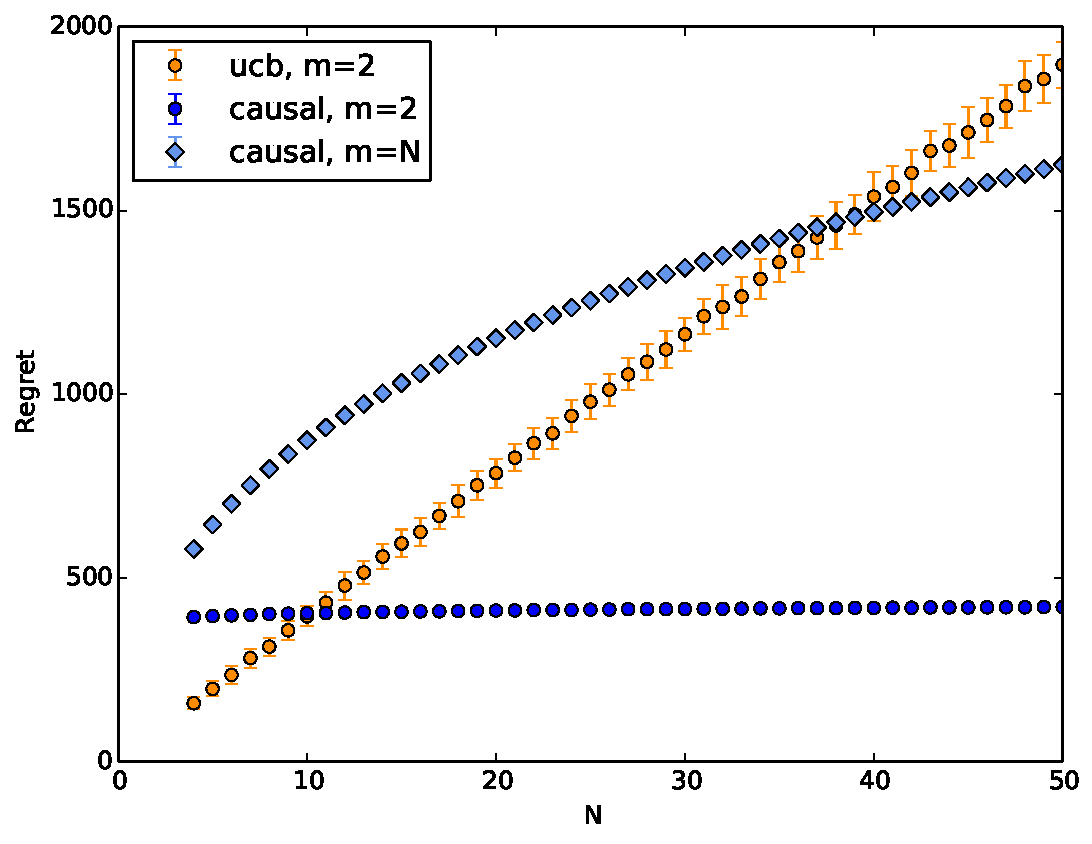
\includegraphics[width=.5\textwidth]{exp_regret_vs_N_T10000_sims100_20151229_113550.pdf}
\end{figure}
\fi

\iffalse
\begin{figure}
\caption{Cumulative regret over time for $N = 17$ for UCB with $\alpha=2$, Causal-Explore-Exploit with $m=2$ and Causal-Explore-Exploit with $m=N$. Shaded region shows standard deviation over 100 simulations. The Causal-Explore-Exploit algorithm incurs linear regret during the exploration phase, after which it selects the optimal arm with high probability. For $m=2$, we have $K \sim m^{2/3}T^{1/3}$ and see that we are in the regime in which Causal-Explore-Exploit outperforms UCB.}
\label{fig:known_q_r_vs_t}
\centering
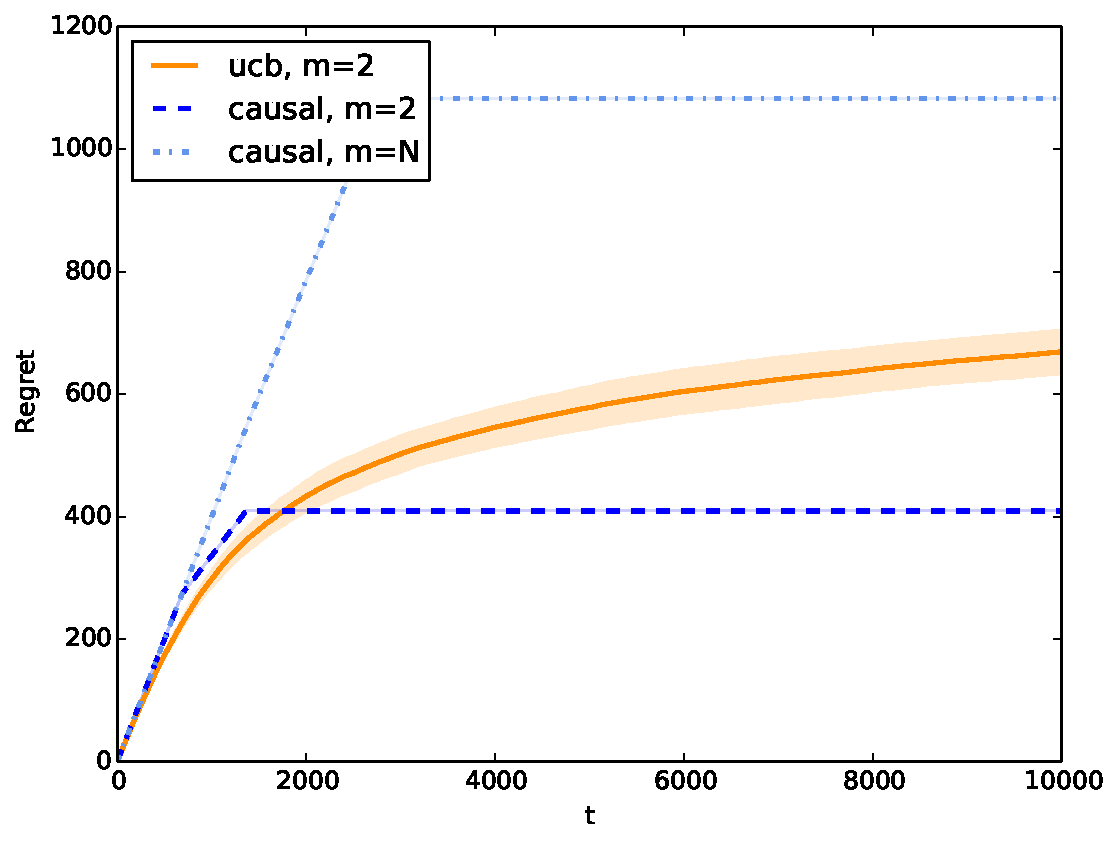
\includegraphics[width=.5\textwidth]{exp_regret_vs_t_T10000_N17_sims100_20151229_120647.pdf}
\end{figure}
\fi

\begin{figure}
\caption{Simple regret vs horizon, $T$, with $N = 20$ and fixed $\epsilon = .4$ for Successive Rejects and Causal-Best-Arm-Identification. Error bars show standard error over 100000 simulations.}
\label{fig:simple_vs_T}
\centering
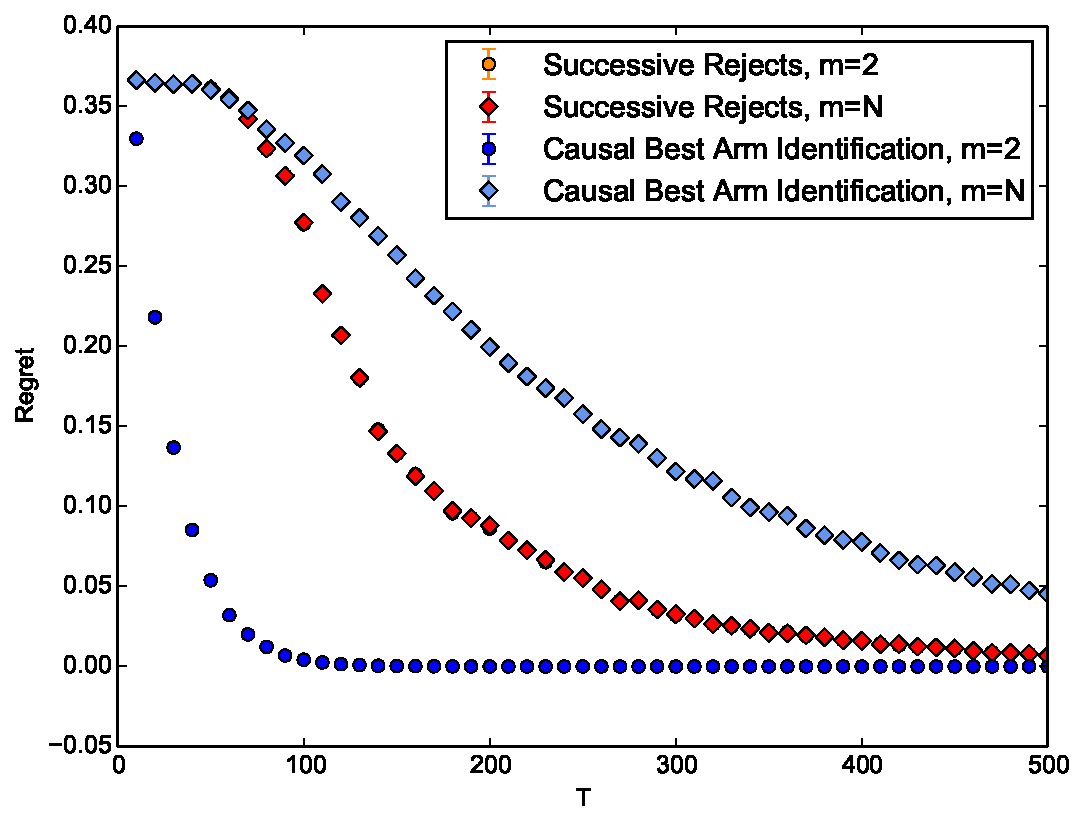
\includegraphics[width=.5\textwidth]{exp_simpleregret_vs_T_N20_sims100000_20160121_140227}
\end{figure}

\begin{figure}
\caption{Simple regret vs horizon, $T$, with $N = 20$ and $\epsilon \propto \sqrt{1/T}$ for Successive Rejects and Causal Best Arm Identification. Error bars show standard error over 10000 simulations.}
\label{fig:simple_vs_T_vary_epsilon}
\centering
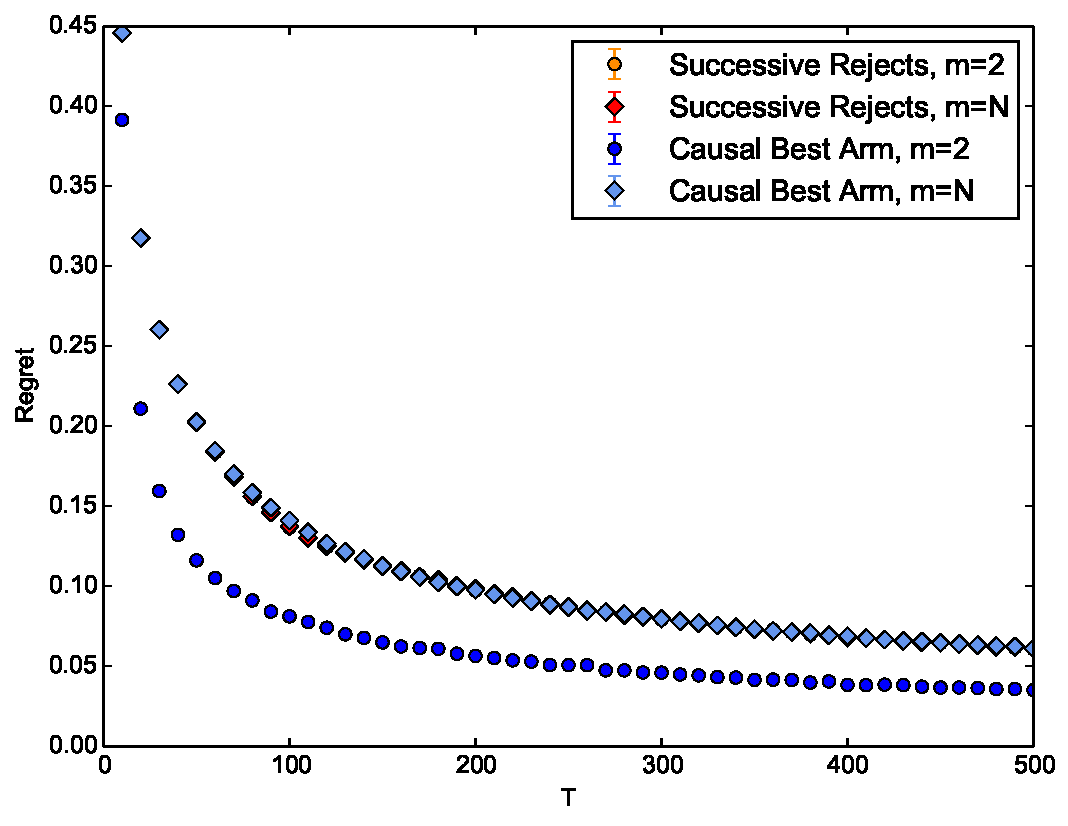
\includegraphics[width=.5\textwidth]{exp_simpleregret_vs_T_N20_sims10000_20160122_010802.pdf}
\end{figure}

\iffalse
\begin{figure}
\caption{Simple regret vs number of variables, $N$, for $T=250$, for Successive Rejects and, Causal-Best-Arm-Identification. Error bars show standard error from 10000 simulations.}
\label{fig:simple_vs_N}
\centering
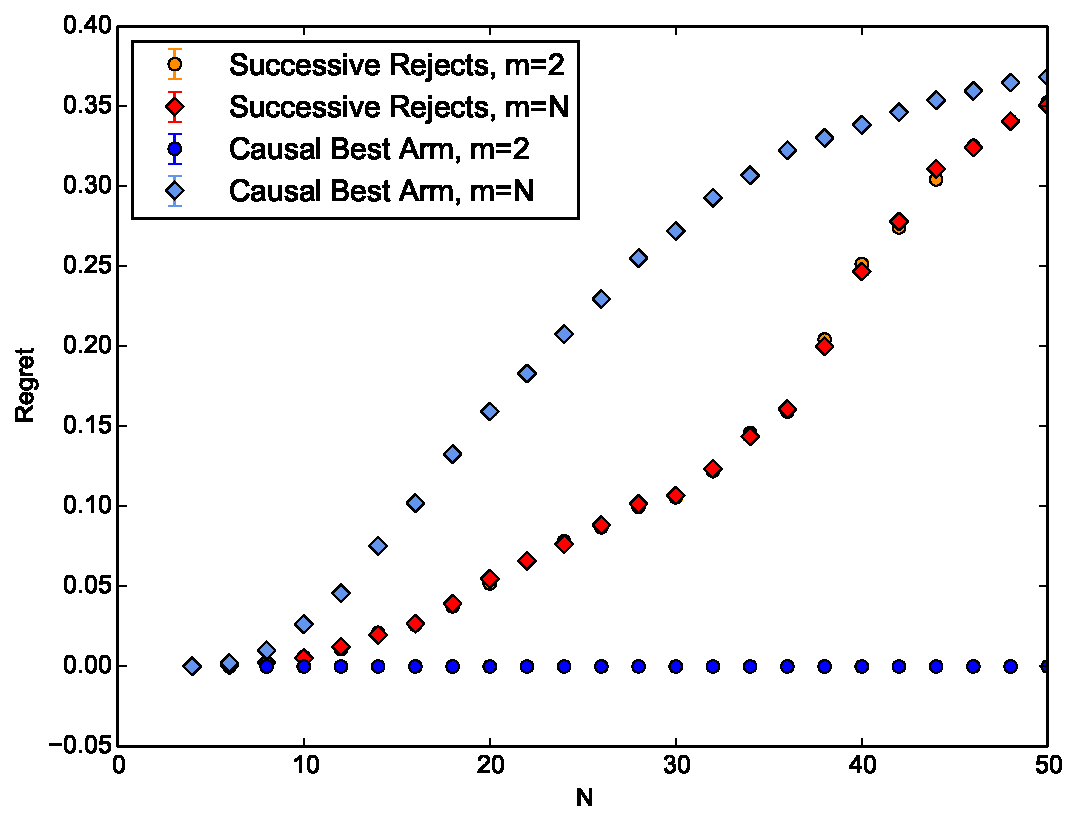
\includegraphics[width=.5\textwidth]{exp_simpleregret_vs_N_T250_sims10000_20160122_024459.pdf}
\end{figure}
\fi


\begin{figure}
\caption{Simple regret vs number of variables, $m$, for $T=300$ and $N = 50$, for Successive Rejects and Causal-Best-Arm-Identification. Error bars show standard error over 10000 simulations.}
\label{fig:simple_vs_m}
\centering
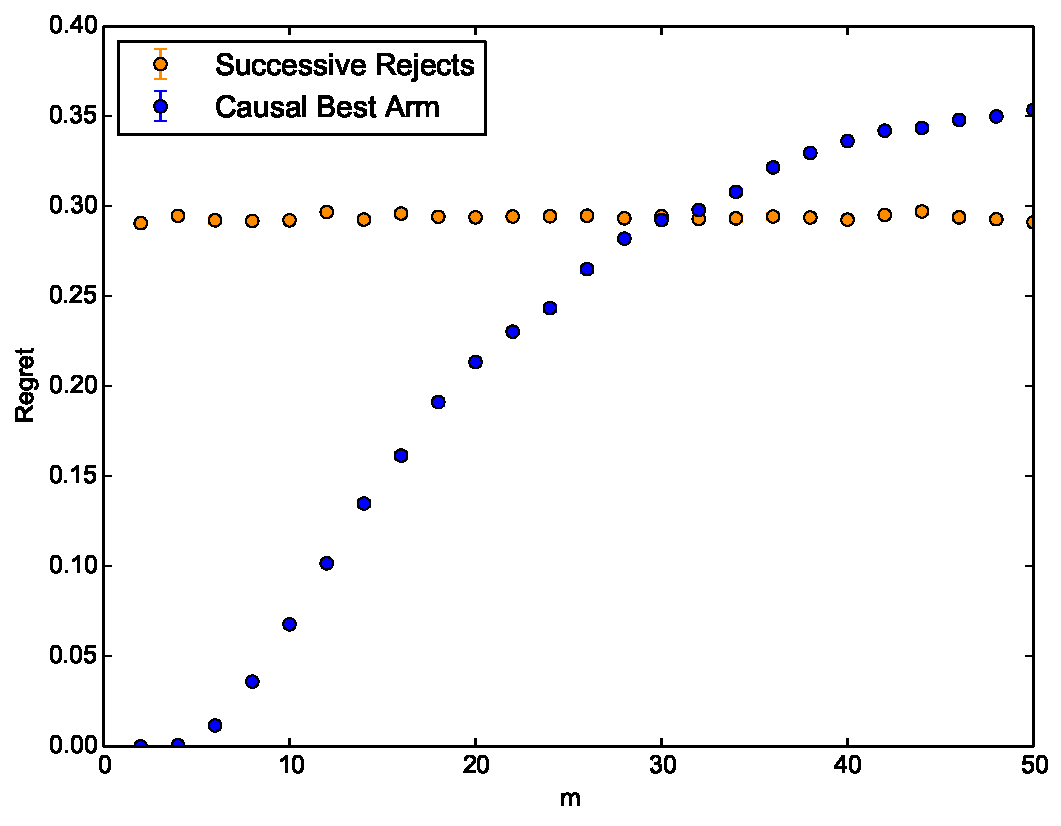
\includegraphics[width=.5\textwidth]{exp_simpleregret_vs_m_T300_N50_sims10000_10000.pdf}
\end{figure}

\iffalse
\begin{figure}
\caption{Simple regret vs number of variables, $N$, for $T=250$, for Successive Rejects and, Causal-Best-Arm-Identification on the confounded bandit problem. Error bars show standard error from 10000 simulations.}
\label{fig:simple_vs_N_confounded}
\centering
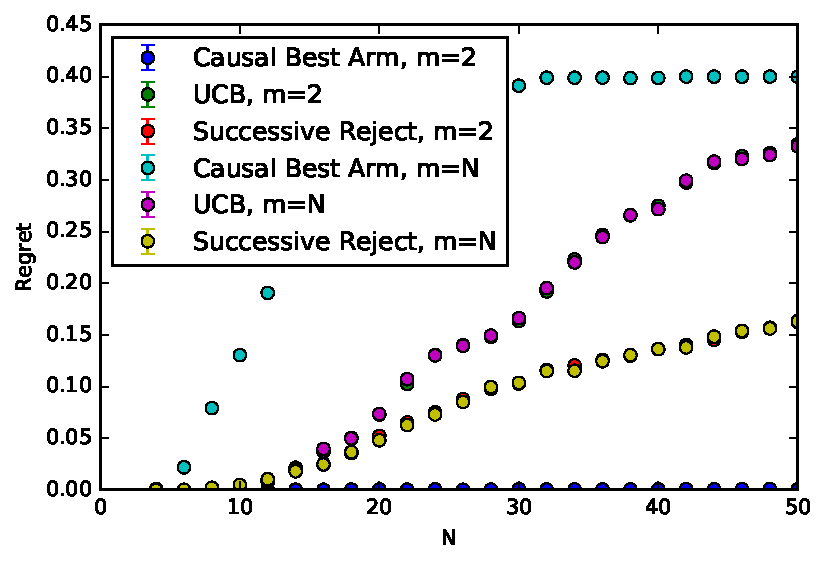
\includegraphics[width=.5\textwidth]{exp_general_simpleregret_vs_N_T250_sims10000_20160131_080208.pdf}
\end{figure}
\fi

\subsection{Experiments on more general graphs}
We now demonstrate the general simple regret algorithm on some graphs that display some interesting behaviour.
 
\begin{figure}[h]
\centering
\caption{Causal model for the confounded bandits problem.}
\label{fig:causalStructure_confounded_N}
\begin{tikzpicture}[->,>=stealth',shorten >=1pt,auto,node distance=1cm,
  thick,main node/.style={observed}, hidden/.style={empty}]
\node[main node](1){$X_{2}$};
\node[main node, right=of 1](2){$X_{3}$};
\node[hidden, right=of 2](3){$...$};
\node[main node, right=of 3](4){$X_{N}$};
\node[main node, below right=of 2](5){Y};
\node[main node,above right=of 2](6){$X_1$}; 
 \path[every node/.style={font=\sffamily\small}]
    (1) edge (5)
    	(2) edge (5)
    (4) edge (5)
    (6) edge (1) edge (2) edge (4);
\end{tikzpicture}
\end{figure}

\subsubsection{X1-dominated confounded model}
A model under which the value of the confounding variable $X_1$ plays the central role in determining $P(Y)$.  Let:
\eq {
\P{Z = 1} &= q \\
\P{X_k = 1|Z=j} &=  q_j \;\; \forall k \in \set{1...n}\\
\P{Y|x_1 ... x_n} &= \bar{\boldsymbol{x}}
} 
This leads to rewards:
\eq {
\P{Y|do(Z = j)} = q^j(1-q)^{1-j}\\
\P{Y|do(X_i = j)} = \begin{cases}
\frac{1}{n} + \frac{n-1}{n}\left(q q_1 + (1-q)q_0 \right) & \text{ if } j = 1 \\
\frac{n-1}{n}\left(q q_1 + (1-q)q_0 \right) & \text { if } j = 0
\end{cases}
}

We can select the probabilities to create a scenario close to the worst case problem such that there is a single arm $do(Z=1)$ that is optimal with expected reward ...

